% This text is proprietary.
% It's a part of presentation made by myself.
% It may not used commercial.
% The noncommercial use such as private and study is free
% May 2007
% Author: Sascha Frank 
% University Freiburg 
% www.informatik.uni-freiburg.de/~frank/
%
% 
\documentclass{beamer}
\setbeamertemplate{navigation symbols}{}

\usepackage{beamerthemeshadow}
\usepackage{algorithm}
\usepackage{float}
\usepackage{algpseudocode}

\begin{document}
\title{Evaluation of hill climbing, simulated annealing, tabu search and random selection: search algorithms
       on cryptographic hash functions BLAKE, Gr{\o}stl and Keccak}  
\author{Soham Sadhu}
\date{\today} 

\begin{frame}
\titlepage
\end{frame}

\begin{frame}
\frametitle{Abstract}
\begin{itemize}
\item In October 2012, Keccak was chosen as the winner of SHA-3 competition amongst 64 candidates, including 
the finalists BLAKE and Gr{\o}stl.
\item I have attempted to find near collisions in reduced versions of BLAKE, Gr{\o}stl and Keccak; using hill
climbing, random selection, simulated annealing and tabu search.
\end{itemize}
\end{frame}

\begin{frame}
\frametitle{Table of contents}
\tableofcontents
\end{frame} 

\section{Introduction}

\subsection{Hash function}
\begin{frame}
  \frametitle{Hash function}
  A \emph{hash family} is a four-tuple ($\mathcal{X}, \mathcal{Y}, \mathcal{K}, \mathcal{H}$),
  satisfying the following conditions.\footnotemark
  \begin{itemize}
    \item $\mathcal{X}$ is a set of possible messages
    \item $\mathcal{Y}$ is a finite set of hash function output
    \item $\mathcal{K}$, the \emph{keyspace}, is a finite set of possible keys
    \item For each $K \in \mathcal{K}$, there is a hash function $h_{k} \in \mathcal{H}$. Each 
      $h_{k}: \mathcal{X} \to \mathcal{Y}$ 
  \end{itemize}
  \footnotetext[1]{Douglas R. Stinson. Cryptography Theory and Practice, chapter 4. Cryptographic
  Hash Functions. Chapman \& Hall/CRC, Boca Raton, FL 33487-2742, USA, third edition, 2006.}
\end{frame}

\subsection{Property of hash function}
\begin{frame}
  \frametitle{Property of Hash function\footnotemark}
  \begin{enumerate}
  \item {\bf Preimage resistance} \\
  {\bf Given:} A hash function $h : \mathcal{X} \to \mathcal{Y}$ and an element $y \in \mathcal{Y}$. \\
  {\bf Find:} $x \in \mathcal{X}$ such that $h(x) = y$.
  \item {\bf Second preimage} \\
  {\bf Given:} A hash function $h : \mathcal{X} \to \mathcal{Y}$ and an element $x \in \mathcal{X}$. \\
  {\bf Find:} $x' \in \mathcal{X}$ such that $x' \neq x$ and $h(x) = h(x')$.
  \item {\bf Collision resistance} \\
  {\bf Given:} A hash function $h : \mathcal{X} \to \mathcal{Y}$ \\
  {\bf Find:} $x, x' \in \mathcal{X}$ such that $x' \neq x$ and $h(x') = h(x)$. 
  \end{enumerate}
  \footnotetext[2]{Douglas R. Stinson. Cryptography Theory and Practice, chapter 4. Cryptographic
  Hash Functions. Chapman \& Hall/CRC, Boca Raton, FL 33487-2742, USA, third edition, 2006.}
\end{frame}

\subsection{Security model}
\begin{frame}
\frametitle{Security model}
\begin{itemize}
\item {\bf Random Oracle} model, proposed by Bellare and Rogaway. Algorithm is secure, modulo the way it creates
the random outputs.\footnotemark
\item {\bf Birthday paradox:} In a sample size of $M$, minimum $N$ number of attempts to find, two elements with
same value is given by equation $N \approx 1.17 \sqrt{M}$. 
\end{itemize}
\footnotetext[3]{Gerrit Bleumer. Random oracle model. In HenkC.A. van Tilborg and Sushil Jajodia,
editors, Encyclopedia of Cryptography and Security, pages 1027–1028. Springer US, 2011.}
\end{frame}

\subsection{Application}
\begin{frame}
\frametitle{Application of hash functions}
\begin{enumerate}
\item {\bf Digital forensics:} take a hash value of evidence, to later prove that it has not been tampered.
\footnotemark
\item {\bf Password stored:} is salted and hased, before inserting to database.
\item {\bf File integrity:} take hash value of files between time intervals, to make sure; they have not
been tampered.
\item {\bf Pseudo random:} generator, based on a seed value.
\end{enumerate}
\footnotetext[4]{Richard P. Salgado. Fourth Amendment Search And The Power Of The Hash, volume
119 of 6, pages 38 – 46. Harvard Law Review Forum, 2006.}
\end{frame}

\subsection{Standards and SHA-3 competition}
\begin{frame}
\frametitle{Standards and SHA-3 competition}
\begin{enumerate}
\item SHA-0 proposed by NSA in 1993, standardised by NIST. In 1995, SHA-0 replaced by SHA-1, designed by NSA.
\footnotemark
\item SHA-1 had block size of 512 bits, size of 160 bits; and additional circular shift operation, to rectify
weakness from SHA-0.
\item SHA-2 designed by NSA, released by NIST in 2001. Family of functions of SHA-224, SHA-256, SHA-384, SHA-512.
\item SHA-3 competition announced on November, 2007. Submissions accepted till October, 2008. From 64 submissions,
that included 5 finalist, Keccak announced as winner on October 2, 2012 by NIST.
\end{enumerate}
\footnotetext[5]{James Joshi. Network Security: Know It All: Know It All. Newnes Know It All.
Elsevier Science, 2008.}
\end{frame}

\section{SHA-3 finalists}

\subsection{BLAKE}

\begin{frame}
\frametitle{BLAKE construction}
BLAKE is built on HAIFA (HAsh Iterative FrAmework) structure \footnotemark which is an improved version of 
Merkle-Damg\.{a}rd function.
\begin{figure}[h]
  \begin{center}
    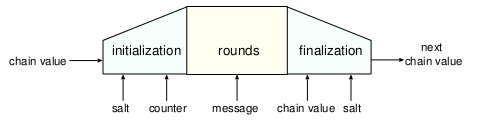
\includegraphics[scale=0.5]{blakelocalwidepipeconstruction.jpg}
  \end{center}
  \caption{Local wide construction of BLAKE's compression function\footnotemark}
  \label{fig:seq}
\end{figure}
\footnotetext[6]{Eli Biham and Orr Dunkelman. A framework for iterative hash functions - haifa.
Cryptology ePrint Archive, Report 2007/278, 2007.}
\footnotetext[7]{Jean-Philippe Aumasson, Luca Henzen, Willi Meier, and Raphael C.-W. Phan. Blake.
http://www.131002.net/blake/blake.pdf, April 2012.}
\end{frame}

\begin{frame}[fragile]
\frametitle{Compression algorithm}
  \begin{algorithm}[H]
  \begin{algorithmic}[1]
    \State $ h^{0} \gets IV $
    \For {$i = 0,\dots, N - 1$}
      \State $h^{i+1} \gets compress(h^{i}, m^{i}, s, l^{i})$
    \EndFor
    \State\Return{$h^{N}$}
  \end{algorithmic}
  \caption[BLAKE Compression]{BLAKE Compression procedure\footnotemark}
  \label{alg:seq}
  \end{algorithm}
  \footnotetext[8]{Jean-Philippe Aumasson, Luca Henzen, Willi Meier, and Raphael C.-W. Phan. Blake.
http://www.131002.net/blake/blake.pdf, April 2012.}
\end{frame}

\subsection{Gr{\o}stl}

\subsection{Keccak}

\end{document}
